\documentclass[12pt, a4paper]{article}
\usepackage[utf8]{inputenc}
\usepackage{physics}
\usepackage{graphicx}
\usepackage{amsmath}
\usepackage{cancel}

\usepackage{MnSymbol}%
\usepackage{wasysym}%
%code color
\usepackage{listings}
\usepackage{xcolor}

\definecolor{codegreen}{rgb}{0,0.6,0}
\definecolor{codegray}{rgb}{0.5,0.5,0.5}
\definecolor{codepurple}{rgb}{0.58,0,0.82}
\definecolor{backcolour}{rgb}{0.95,0.95,0.92}

\lstdefinestyle{mystyle}{
	backgroundcolor=\color{backcolour},   
	commentstyle=\color{codegreen},
	keywordstyle=\color{magenta},
	numberstyle=\tiny\color{codegray},
	stringstyle=\color{codepurple},
	basicstyle=\ttfamily\footnotesize,
	breakatwhitespace=false,         
	breaklines=true,                 
	captionpos=b,                    
	keepspaces=true,                 
	numbers=left,                    
	numbersep=5pt,                  
	showspaces=false,                
	showstringspaces=false,
	showtabs=false,                  
	tabsize=2
}

\lstset{style=mystyle}

\begin{document}
	Mr. Phiphat Chomchit 630631028
	\begin{center}
		\textbf{ Grover’s Search (10/11/2021)}
	\end{center}
	\begin{enumerate}
		\item Grover algorithm implementation for $N = 4$ and target $\ket{00}.$
			\begin{lstlisting}[language=Java, caption= Oracle |00>]
			OPENQASM 2.0;
			include "qelib1.inc";
			qreg q[2];
			creg c[2];
			
			h q;
			
			//Oracle |00>
			x q;
			h q[1];
			cx q[0], q[1];
			h q[1];
			x q;
			
			//Grover's diffusion
			h q;
			x q;
			h q[1];
			cx q[0], q[1];
			h q[1];
			x q;
			h q;
			
			measure  q -> c;
			
		\end{lstlisting}
		
		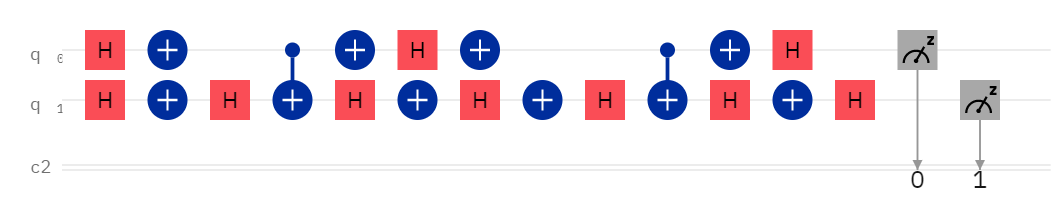
\includegraphics[scale=0.4]{circuit-00.png}
		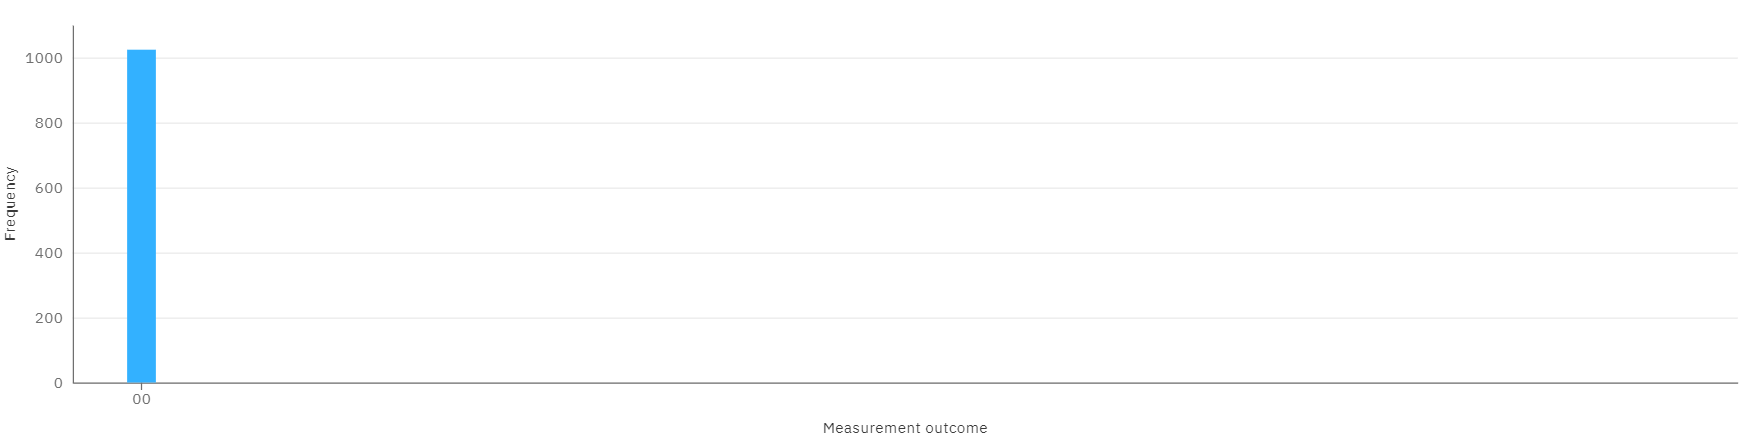
\includegraphics[scale=0.2]{bar-00.png}
		
		\item Grover algorithm implementation for $N = 4$ and target $\ket{01}.$
		\begin{lstlisting}[language=Java, caption= Oracle |01>]
			OPENQASM 2.0;
			include "qelib1.inc";
			qreg q[2];
			creg c[2];
			
			h q;
			
			//Oracle |01>
			x q[1];
			h q[1];
			cx q[0], q[1];
			h q[1];
			x q[1];
			
			//Grover's diffusion
			h q;
			x q;
			h q[1];
			cx q[0], q[1];
			h q[1];
			x q;
			h q;
			
			measure  q -> c;
			
		\end{lstlisting}
		
		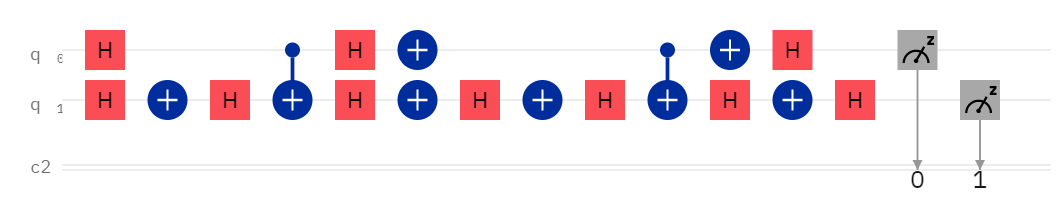
\includegraphics[scale=0.4]{circuit-01.png}
		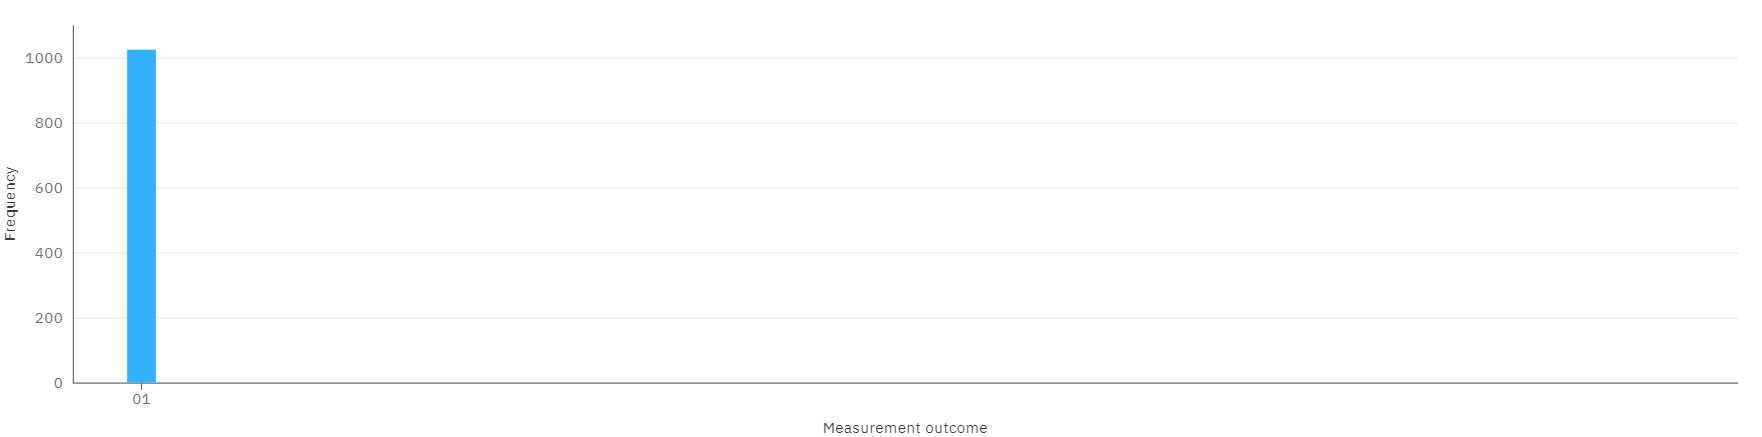
\includegraphics[scale=0.2]{bar-01.png}
		\newpage
		\item Grover algorithm implementation for $N = 4$ and target $\ket{11}.$
		\begin{lstlisting}[language=Java, caption= Oracle |11>]
			OPENQASM 2.0;
			include "qelib1.inc";
			qreg q[2];
			creg c[2];
			
			h q;
			
			//Oracle |11>
			h q[1];
			cx q[0], q[1];
			h q[1];
			
			//Grover's diffusion
			h q;
			x q;
			h q[1];
			cx q[0], q[1];
			h q[1];
			x q;
			h q;
			
			measure  q -> c;
			
		\end{lstlisting}
		
		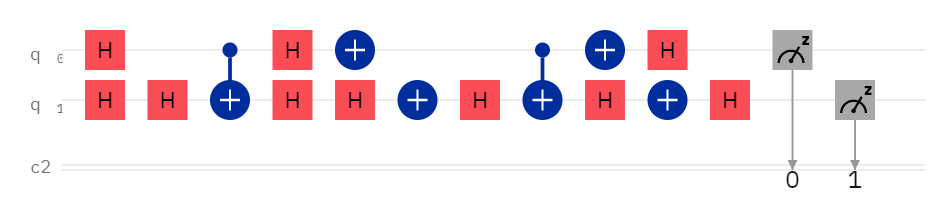
\includegraphics[scale=0.4]{circuit-11.png}
		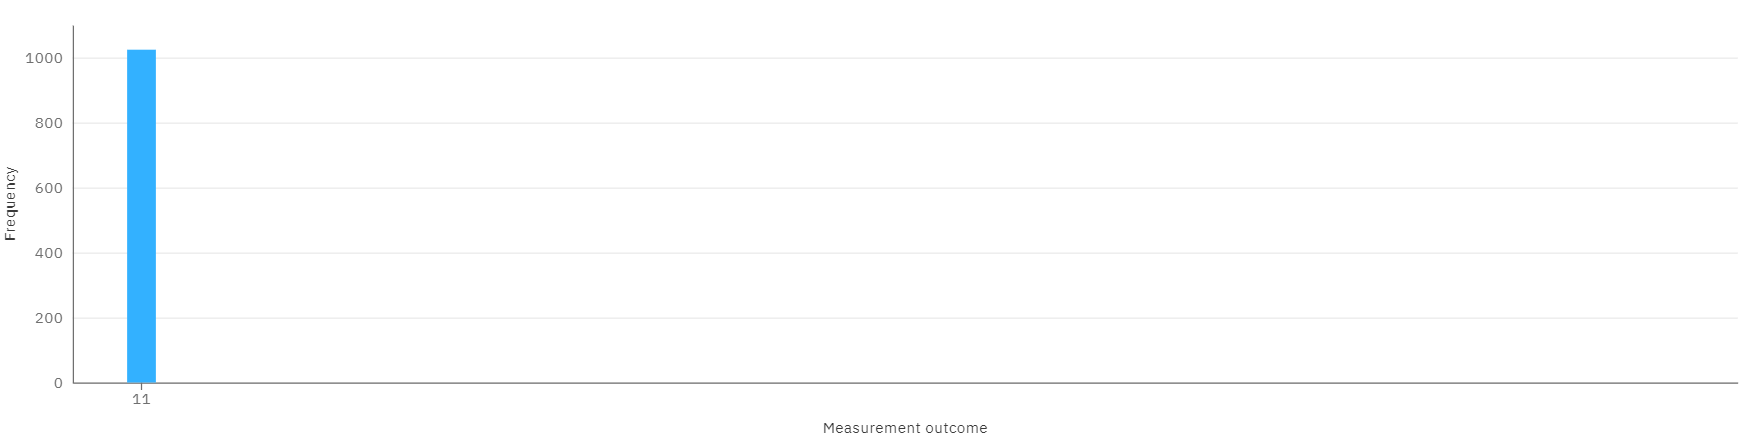
\includegraphics[scale=0.2]{bar-11.png}
	\end{enumerate}
\end{document}
